\RequirePackage{shellesc}
\immediate\write18{cd ..; tex spath3_code.dtx}
\documentclass{article}
\usepackage{tikz}
\usetikzlibrary{
  knots,
  hobby,
  celtic,
  decorations.pathreplacing,
  shapes.geometric,
  calc
}
\usepackage{braids}

\tikzset{
  knot diagram/every strand/.append style={
    ultra thick,red
  },
  show curve controls/.style={
    postaction=decorate,
    decoration={show path construction,
      curveto code={
        \draw [blue, dashed]
        (\tikzinputsegmentfirst) -- (\tikzinputsegmentsupporta)
        node [at end, draw, solid, red, inner sep=2pt]{};
        \draw [blue, dashed]
        (\tikzinputsegmentsupportb) -- (\tikzinputsegmentlast)
        node [at start, draw, solid, red, inner sep=2pt]{}
        node [at end, fill, blue, ellipse, inner sep=2pt]{}
        ;
      }
    }
  },
  show curve endpoints/.style={
    postaction=decorate,
    decoration={show path construction,
      curveto code={
        \node [fill, blue, ellipse, inner sep=2pt] at (\tikzinputsegmentlast) {}
        ;
      }
    }
  }
}

\begin{document}

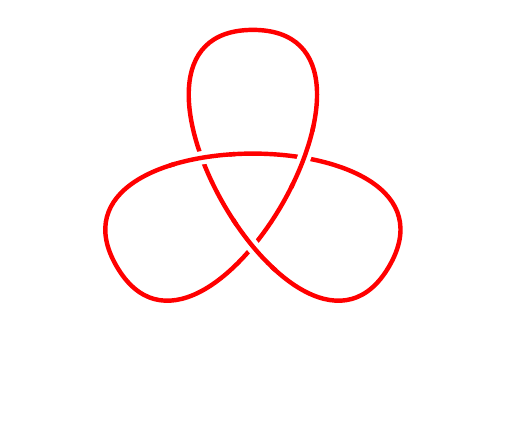
\begin{tikzpicture}
\begin{knot}[
  consider self intersections=true,
%  draft mode=crossings,
  flip crossing={2},
  only when rendering/.style={
    spath/show current path,
  }
]
\strand (0,2) .. controls +(2.2,0) and +(120:-2.2) .. (210:2) .. controls +(120:2.2) and +(60:2.2) .. (-30:2) .. controls +(60:-2.2) and +(-2.2,0) .. (0,2);
\end{knot}
\end{tikzpicture}

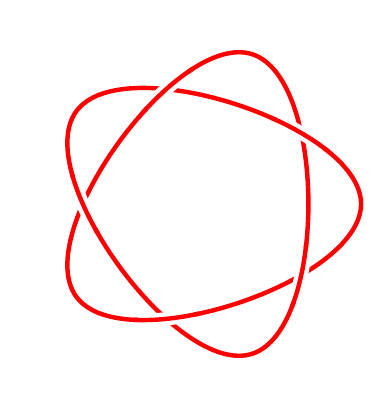
\begin{tikzpicture}
\begin{knot}[
  consider self intersections=true,
%  draft mode=crossings,
  flip crossing/.list={2,4},
  only when rendering/.style={
%    show curve controls
  }
]
\strand (2,0) .. controls +(0,1.0) and +(54:1.0) .. (144:2) .. controls +(54:-1.0) and +(18:-1.0) .. (-72:2) .. controls +(18:1.0) and +(162:-1.0) .. (72:2) .. controls +(162:1.0) and +(126:1.0) .. (-144:2) .. controls +(126:-1.0) and +(0,-1.0) .. (2,0);
\end{knot}
\end{tikzpicture}

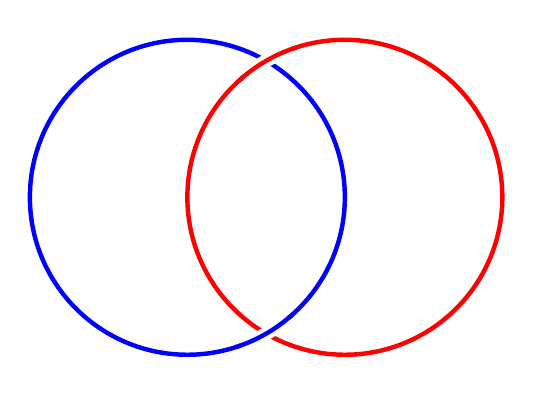
\begin{tikzpicture}
\begin{knot}[
%  draft mode=crossings,
  flip crossing=2
]
\strand (1,0) circle[radius=2cm];
\strand[blue] (-1,0) circle[radius=2cm];
\end{knot}
\end{tikzpicture}

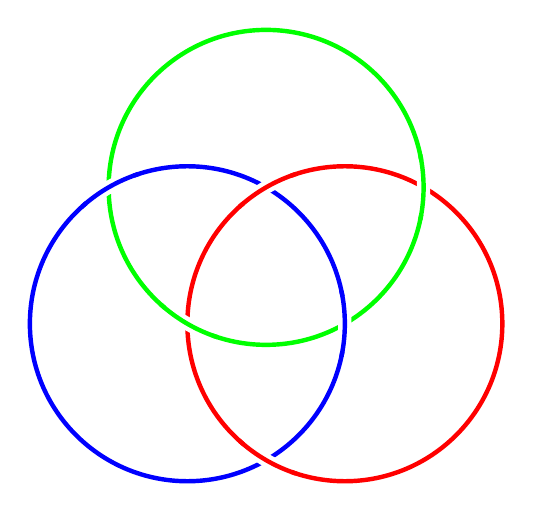
\begin{tikzpicture}
\begin{knot}[
%  draft mode=crossings,
  flip crossing/.list={3,4}
]
\strand (1,0) circle[radius=2cm];
\strand[blue] (-1,0) circle[radius=2cm];
\strand[green] (0,{sqrt(3)}) circle[radius=2cm];
\end{knot}
\end{tikzpicture}


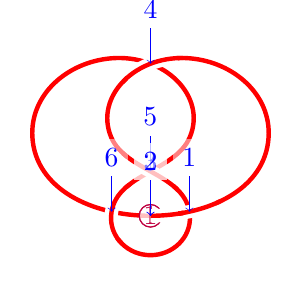
\begin{tikzpicture}[use Hobby shortcut]
\begin{knot}[
  consider self intersections=true,
  draft mode=crossings,
  ignore endpoint intersections=false,
%  flip crossing=3
]
\strand ([closed]0,0) .. (1.5,1) .. (.5,2) .. (-.5,1) .. (.5,0) .. (0,-.5) .. (-.5,0) .. (.5,1) .. (-.5,2) .. (-1.5,1) .. (0,0);
\end{knot}
\path (0,-.7);
\end{tikzpicture}

\end{document}
